\chapter{Theory: Neural dynamics}
\label{sec:Neuron}
\index{Multicompartmental neuron model}
The main contribution to extracellular potentials comes from the electrical activity of neurons. To model extracellular potentials, we therefore first need a model of the neurons generating them. Moreover, a neuron's contribution to the extracellular potential depends strongly on its morphology, 
meaning that we will need multicompar\ehtxt{t}mental 
neuron models \index{Multicompartment model} that account for the neuron's spatial extension.

Modeling of neurons is at the core of computational neuroscience. There exist many types of frameworks for constructing neuronal models at various levels of detail and abstraction, and the topic has been treated in detail in several text books (see e.g.,\cite**{johnston1994foundations,KockSegev1998,Koch1999,DeSchutter2000,Hille2001,Dayan2005,Izhikevich2007,Sterratt2011,Miller2018}). We shall here give only a rather brief introduction to the topic, and we shall limit ourselves to present the most standard kind multicompartmental neuron model, based on a framework which combines a so-called Hodgkin-Huxley type description of the neural membrane mechanisms (see e.g., \cite**{Hodgkin1952,KockSegev1998,Pospischil2008}) with cable theory to predict how signals propagate spatially in dendrites and axons (see, e.g., \cite**{Koch1999,rall2011}). We shall refer to this framework simply as the multicompartment (MC) framework. The MC framework has become the gold standard for biophysically detailed neuronal simulations on the cellular and network level, and has been used for simulating the dynamics of large neuronal networks (see e.g., \cite**{traub2005,markram2015,arkhipov2018}).

A MC model is characterized by (i) its morphology, and (ii) its membrane mechanisms, and the key dynamical variable is the membrane potential (V). The morphology (i) of the real neuron (Fig. \ref{Neuron:fig:multicomp}A) is represented as a discretized set of compartments connected by resistors (Fig. \ref{Neuron:fig:multicomp}B), and there are two categories of currents which together determine the membrane potential dynamics in the compartments (Fig. \ref{Neuron:fig:multicomp}C). These are the currents that run intracellularly between compartments (yellow arrows), and the transmembrane currents at each compartment (green arrows), which are determined by a set of (ii) neuron specific membrane mechanisms. Once all the currents are characterized, the dynamics of the membrane potential can be computed by Kirchhoff's current law, which demands that the sum of currents into a given compartment is zero.

\begin{figure}[!ht]
\begin{center}
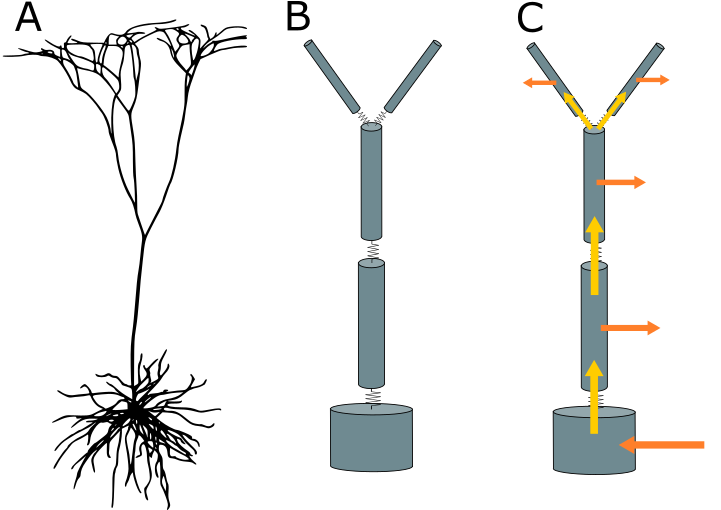
\includegraphics[width=0.6\textwidth]{Figures/Neuron/multicompartment.png}
\end{center}
\caption{\textbf{Multicompartmental modelling.}  (A) The neural morphology is (B) represented by a multicompartmental model, where the compartments are treated as cylinders connected by resistors. The example shows a crudely simplified model containing only five compartments, but detailed multicompartment models may include several hundreds of compartments, and can represent t he morphology in great detail. (C) Electric currents in the model can be separated into two groups: (i) transmembrane current in a compartment (green arrows), and (ii) intracellular currents between compartments (yellow arrows). 
}
\label{Neuron:fig:multicomp}
\end{figure}

To present the MC framework, we will start by presenting a framework for modeling the transmembrane currents in a single compartment (Section \ref{sec:Neuron:membranecurrents}), and next show how a number of such compartments can be connected together to a MC model (Section \ref{sec:Neuron:morphology}). Together, those two sections provide a theoretical framework for modeling neurons that should be sufficient for most practical applications. Readers that crave further biophysical insight into the ionic movements that actually give rise to the transmembrane neural currents can get a brief introduction to this in Section\ref{sec:Neuron:Ions_and_reversals}. Finally, we end the chapter about neuronal modeling by briefly summarizing the main assumptions underlying the HHC (Section \ref{sec:Neuron:HHCassumptions}).


\section{\blue{Membrane currents}}
\label{sec:Neuron:membranecurrents}
\index{Hodgkin-Huxley type model}
Hodgkin-Huxley (HH) type models are called so because they describe the membrane mechanisms with a mathematical formalism similar to that used in celebrated model by \citeasnoun**{Hodgkin1952}. In HH-type models, the membrane typically includes three autonomous classes of transmembrane currents, normally represented as current densities (unit mA/cm$^2$). These are (i) a capacitive current density ($i_c$), (ii) a the leakage current density ($i_L$), and (iii) a the current density through active ion channels ($i_x$), of which there may be several different kinds ($x$ is an index). 
\ehnote{Notasjon boer ryddes opp i. Kursiv subfix boer representere index, mens subfix som er en forkortelse (c-capacitance, m-membrane etc.) skal ikke vaere kursiv men normal font: $i_\mathrm{m}$.}
In addition, a neuron may receive  (iv) external stimuli ($i_{stim}$) either through synaptic currents or experimental current injections. In the case where the neuron is modeled as a single compartment, the net transmembrane current must be zero, so that:

\begin{equation}
i_c + i_L + \sum_x{i_x} +  i_{stim} = 0.
\label{Neuron:eq:singlecomp_zerosum}
\end{equation}
Below, we define the various currents that go into this equation.


\subsection{\blue{Capacitive current}}
\label{sec:Neuron:Cap}
\index{Capacitive current}

The capacitive current density,
\begin{equation}
i_c = c_m \frac{dV}{dt},
\label{Neuron:eq:HHcap}
\end{equation}
represents the charging up of the membrane potential $V$ due to a charge density accumulating on the outside of inside of the capacitive membrane. Here, $c_m$ is the specific membrane capacitance. In the original HH-model, $c_m$ had the value
1 $\mu$F/cm$^2$, and this value seems to be representative for most neurons.  An illustration of how to interpret the capacitive current is given in Fig. \ref{Neuron:fig:capacitive_currents}. 

\begin{figure}[!ht]
\begin{center}
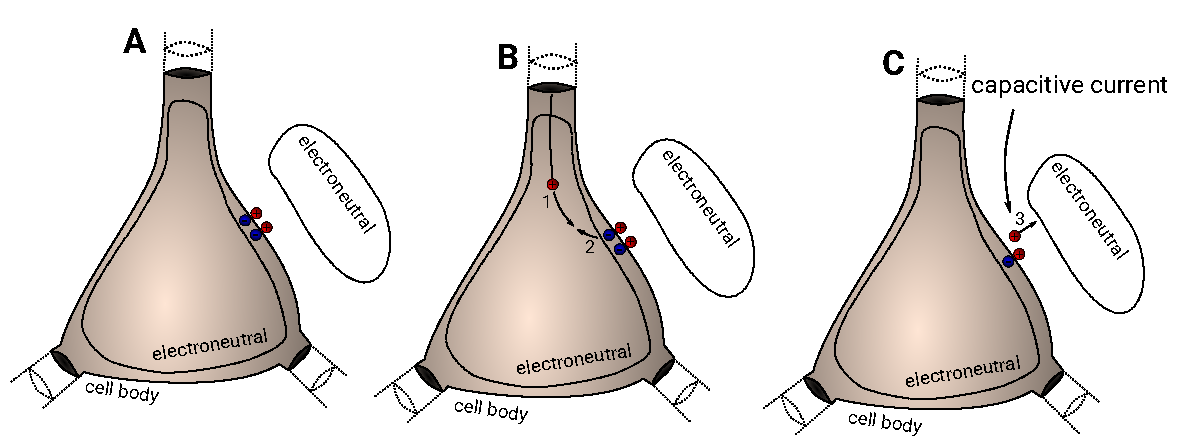
\includegraphics[width=0.8\textwidth]{Figures/Neuron/capacitive_currents.pdf}
\end{center}
\caption{\textbf{Capacitive currents are important for current conservation.}  (\textbf{(A)}) The extracellular and intracellular bulk solutions are essentially electroneutral, and the only region where there is a nonzero charge density is in thin Debye layers around the capacitive membrane. Unlike the other currents involved, the capacitive current is not due to ions crossing the membrane, but due to ions piling up on either side of it, separating a membrane charge density $\eta$ and a charge membrane charge density $-\eta$, giving rise to a membrane potential of $V = \eta/c_m$. An outward capacitive current could correspond to an anion leaving the membrane on the inside (\textbf{(B)}), which will coincide with a cation leaving the membrane on the outside (\textbf{(C)}). Thus, capacitive membrane currents do give rise to electrical ionic volume currents both in the intra- and extracellular space.
}
\label{Neuron:fig:capacitive_currents}
\end{figure}

If we insert eq. \ref{Neuron:eq:HHcap} into eq. \ref{Neuron:eq:singlecomp_zerosum}, we get:
\begin{equation}
c_m \frac{dV}{dt} = - (i_L + \sum_x{i_x} +  i_{stim}),
\label{Neuron:eq:singlecomp_capinserted}
\end{equation}
which may give us an intuitive understanding of neurodynamics: If the sum of ionic currents over the membrane (right hand side) is nonzero, it will lead to a charging up (left hand side) of the membrane. 


\subsection{\blue{Leakage current}}
\label{sec:Neuron:leak}
\index{Leakage current}

The leakage current density is given by
\begin{equation}
i_L = \bar{g}_L (V - E_L),
\label{Neuron:eq:HHleak}
\end{equation}
where $\bar{g}_L$ (mS/cm$^2$) is the leak conductance (the bar indicates that it's a constant). The factor $(V - E_L)$ (mV) is often called the driving force, and $E_L$ the leak reversal potential. The biophysical origin of the reversal potential is explained later (see Section \ref{sec:Neuron:Ions_and_reversals}). For now, we may simply think of $E_L$ as the "target potential" that the leakage current will strive to drive the membrane potential towards. In reality, the leakage current is not a single current, but represents an orchestra of physiological processes that together will drive the membrane potential towards the value $E_L$. 

Together, the capacitive current and the leakage current determine the passive properties of the membrane. If the neuron were to include only these two currents, it could be well modeled as an RC-circuit, and RC-neuron models are often used to simulate the subthreshold dynamics of neurons (Fig. \ref{Neuron:fig:RC}). 

\begin{figure}[!ht]
\begin{center}
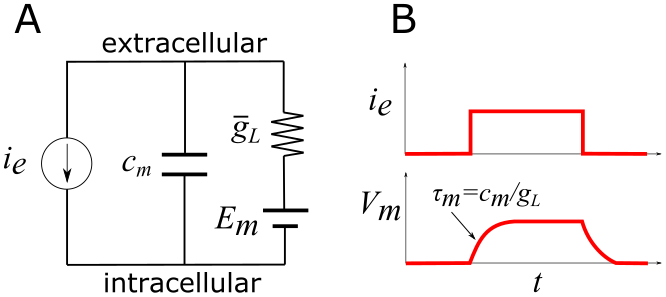
\includegraphics[width=0.8\textwidth]{Figures/Neuron/RCneuron.png}
\end{center}
\caption{\textbf{RC-neuron.}  A neuron model containing only a capacitive and a leakage current can be represented as an RC-circuit. To use standard MC modeling convention, we we have expressed the various variables and parameters in units per membrane area: With a total membrane resistance $R = 1/(g_L A)$, and capacitance $C = c_mA$, we get that $RC = c_m/g_L$. In the illustration, the neuron is given a current injection $i_e$ (A/cm$^2$) and responds by charging up the membrane. When the input is terminated, the membrane potential will return to the value $E_L$. In the RC-model, $E_L$ will be identical to the resting potential of the neuron, i.e., the potential that the membrane will settle on in the case where it does not receive any input. In models which include additional, active ion channels, these can in principle affect the resting potential, so that it may generally differ from $E_L$.
}
\label{Neuron:fig:RC}
\end{figure}


\subsection{\blue{Active ion channels}}
\label{sec:Neuron:active}
\index{Active ion channels}
In addition to $i_c$ and $i_L$, biophysical neuronal models typically include a number of active ion channels. These account for the "fancy" aspect of neurodynamics, and the main legacy of Hodgkin and Huxley was that they derived a mathematical model for describing the kinetics of these \cite**{Hodgkin1952}.

In the HH-type formalism, the current through an active ion channel type $x$ is modeled as:
\begin{equation}
i_x = \bar{g}_x m_x^{\alpha} h_x^{\beta}(V-E_x).
\label{Neuron:eq:HHform}
\end{equation}
We note that the current density $i_x$ does not represent the current through a single ion channel, but a large number of channels of the same type $x$. Thus, $\bar{g}_x$ (mS/cm$^2$) denotes the conductance when all channels of type $x$ are fully open (the bar indicates that it's a constant), while $E_x$ (mV) is the reversal potential for the ion species that travels through the channel type. In analogy with the leak reversal potential, we may think of $E_x$ as the target potential that the current through ion channel $x$ will strive to drive the membrane potential towards. The intrinsic membrane potential dynamics is thus due to the competition between various currents that try to drive it towards their respective reversal potentials. 

If one prefers to think of neurons in terms of circuit diagrams, the active ion channels are simply added in parallel to the passive $i_c$ and $i_L$ currents. As an example, the electric circuit representation of the HH model is depicted in Fig. \ref{Neuron:fig:HH}.

\begin{figure}[!ht]
\begin{center}
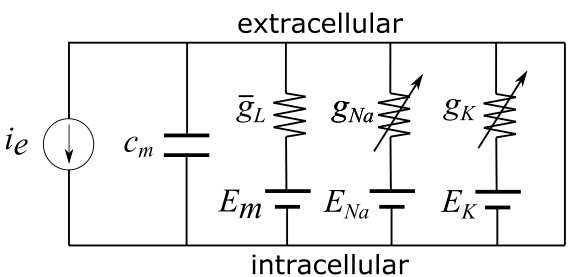
\includegraphics[width=0.8\textwidth]{Figures/Neuron/HHmodel.png}
\end{center}
\caption[]{\textbf{Active, single compartment neuron model.}  In addition to a capacitive and a leakage current, active neuron models contain a number of active ion channels. The example diagram shows the original Hodgkin-Huxley model, with an active Na$^+$ and an active K$^+$ channel. The arrows slicing the diagram conductances indicate that they are variables.}
\label{Neuron:fig:HH}
\end{figure}

Active ion channels differ from the passive leakage channel in that their total conductance, $\bar{g}_{x} m^{\alpha} h^{\beta}$, vary with time due to the so-called gating variables, in eq. \ref{Neuron:eq:HHform} denoted $m$ and $h$. These determine the dynamics of how the ion channels activate or deactivate (open or close), and $m$ and $h$ represent two different types of gates differing in terms of their opening/closing dynamics. The exponents $\alpha$ and $\beta$ represent the number of copies that a channel $x$ has of each type of gate. At the level of a single ion channel the values of $m$ and $h$ would interpret as the \textit{probability} that a given gate is in the open state. However, as we here deal with summed currents through a large number of ion channels, the values of $m$ and $h$ interpret as the \textit{fraction} of the gates of the various types that are open. The values are thus numbers between 0 (all gates in the closed state) and 1 (all gates in the open state). The product $m^{\alpha} h^{\beta}$ thus interprets as the fractions of ion channels in which all gates are open so that currents can pass through. The ion channel conductance is thus given by the product $\bar{g}_x m_x^{\alpha} h_x^{\beta}$.

For voltage-gated ion channels, the the dynamics of the gating variables can be described by kinetics equations on the form:
\begin{equation}
\frac{dx(V,t)}{dt} = \frac{x_{\infty}(V) - x}{\tau_x(V)},  \, \text{for } x = \{m,h\}.
\label{Neuron:eq:HHgate}
\end{equation}
Here, the steady state activation $x_{\infty}(V)$, represents the fraction of gates that will end up in the open state if the cell is clamped at a given potential $V$ for sufficiently long time. However, the process of opening the gates takes some time, as accounted for by the activation time constant $\tau_x(V)$ (ms). Both $x_{\infty}(V)$ and $\tau_x(V)$ are functions of the membrane potential, and these must be determined experimentally for each individual ion channel type. We do not go into the experimental challenges here, but will think of them as known functions. 

There are also many ion channels whose activation or inactivation do not depend on $V$, but on some other variable, such as the concentration of some ion species or ligand \cite**{Hille2001,Sterratt2011}. A common example are Ca$^{2+}$ gated ion channels, i.e., channels with gate opening controlled by the intracellular Ca$^{2+}$ concentration ($[Ca^{2+}]_i$). There are also ion channels whose activation depend on more than one variable, such as e.g., ion channels whose activation depend on both $V$ and $[Ca^{2+}]_i$. Fortunately, a HH type formalism can in most cases be applied also to these kind of ion channels, provided that $x_{\infty}(V)$ and $\tau_x(V)$ in eq. \ref{Neuron:eq:HHgate} can be replaced with experimentally determined functions of the relevant variables \cite**{Sterratt2011}. 

To give an example of an active neuron model, the full set of equations for the HH model is summarized in Box \ref{Neuron:box:HH}. Compared to modern biophysically detailed neuron models, the original Hodgkin-Huxley model is relatively simple in that it only contains two (voltage-gated) active ion channels, a Na$^+$ with three activation gates ($m^3$) and one inactivation gate ($h$), as well as a K$^+$ channel with four inactivation gates $n^4$. The two active ion channels are together responsible for action potential generation.  

\begin{floatingbox}[h]
\caption{Hodgkin-Huxley equations}

\begin{eqnarray*}
    c_m \frac{dV}{dt} & =  & -\bar{g}_L(V-E_L) - \bar{g}_{Na} m^3 h (V - E_{Na}) - \bar{g}_{K} n^4 (V - E_{K}) \\
    \frac{dx(V,t)}{dt} & = & \frac{x_{\infty}(V) - x}{\tau_x(V)},  \, \text{for } x = \{m,h,n\} \\ 
    x_{\infty}(V) &= & \frac{\alpha_x(V)}{\alpha_x(V) + \beta_x(V)}, \, \text{for } x = m,n,h \\ %\hline
    \tau_x(V) & = & \frac{1}{\alpha_x(V) + \beta_x(V)}, \, \text{for } x = m,n,h \\ %\hline
    \alpha_n &=& \frac{0.01 \mathrm{ms}^{-1} V+55 \mathrm{mV}}{1-e^{-(V+55 \mathrm{mV})/10 \mathrm{mV}}}  \\ %\hline
     \beta_n &=& 0.125 \mathrm{ms}^-1 e^{-(V+65 \mathrm{mV})/80 \mathrm{mV}}   \\ %\hline
     \alpha_m &=& \frac{0.1 \mathrm{ms}^{-1} V+ 40 \mathrm{mV}} {1-e^{-(V+40 \mathrm{mV})/10 \mathrm{mV}}}  \\   
     \beta_m &=& 4 \mathrm{ms}^{-1} e^{-(V+65  \mathrm{mV})/18 \mathrm{mV}}  \\ %\hline
    \alpha_h &=& 0.07 \mathrm{ms}^{-1} e^{-(V+65 \mathrm{mV})/20 \mathrm{mV}}  \\ %\hline
    \beta_h &=& \frac{1 \mathrm{ms}^{-1}}{1+e^{-(V+35 \mathrm{mV}))/10 \mathrm{mV})}}   \\ %\hline
    c_m &=& 1.0 \mathrm{\mu F/cm^2} \\ %\hline
    \bar{g}{Na} &=& 120 \mathrm{mS/cm^2}\\ %\hline
    \bar{g}_{K} &=& 36 \mathrm{mS/cm^2} \\ %\hline
    \bar{g}_{L} &=& 0.3 \mathrm{mS/cm^2} \\ %\hline
    E_{Na} &=& 50 \mathrm{mV} \\ %\hline
    E_{K} &=& -77  \mathrm{mV} \\ %\hline
    E_{L} &=& -54.4 \mathrm{mV} \\ %\hline
\end{eqnarray*}
\label{Neuron:box:HH}
\end{floatingbox}




\subsection{\blue{Stimulus currents and synapses}}
\label{sec:Neuron:stim}
\index{Stimulus currents}
Finally, the stimulus current in Eq. \ref{Neuron:eq:singlecomp_zerosum}, can represent any external stimulus that a neuron receives. Typically, it is either taken to represent an experimental current injection such as for example a step-current injection:

\begin{equation}
i_\text{inj}(x)= 
\begin{cases}
    constant, & \text{if } t_{start} > t > t_{end} \\
    0,              & \text{otherwise},
\end{cases}
\label{Neuron:eq:injected}
\end{equation}
or a synaptic input. 

The most common synapses are chemical synapses, which are normally modeled more or less like an ion channel:
\begin{equation}
i_\text{syn}(t) = g_\text{syn}(t) \big(V(t)-E_\text{syn} \big), 
\label{Neuron:eq:chemicalsynapse}
\end{equation}
where $E_\text{syn}$ is the reversal potential of the synapse, and $g_\text{syn}(t)$ the conductance. 

The value of $E_\text{syn}$ determines whether a synapse is \textit{excitatory}, which means that it will tend to drive the  membrane potential of neuron toward the threshold for generating action potentials, or \textit{inhibitory}, which means that it will tend to drive the neuron away from the threshold for generating action potentials. Examples of excitatory synapses are AMPA and NMDA synapses, in which $E_\text{syn}$ ($\sim$ 0 - 10 mV) is high above the neuronal resting potential. The most common inhibitory synapse, is the GABA synapse, in which $E_\text{syn}$ ($\sim$ - 70 mV) is close to the resting membrane potential of the neuron.

Unlike for ion channels, which are often voltage or calcium activated, the chemical synapse is activated by neurotransmitters received from a pre-synaptic cell. However, the synaptic response tends to be rather stereotypical, meaning that the post-synaptic response is more or less the same every time the synapse is activated. It is therefore not common to model neurotransmitter activation explicitly. Instead, $g_\text{syn}(t)$ is normally modeled simply as a constant $\bar{g}_\text{syn}$ multiplied with a temporal kernel determining the opening and closing of a synapse set off at an activation time $t_s$. 

Typical choices for $g_\text{syn}(t)$ are \index{Synapse models}: 
\begin{align}
&\text{(i) exponential decay:} \;\; g_\text{syn}(t) = \bar{g}_\text{syn} e^{-(t-t_\text{s})/\tau}\, \Theta(t-t_\text{s}) \\
&\text{(ii) $\alpha$-function:} \;\; g_\text{syn}(t) = \bar{g}_\text{syn} \frac{t-t_\text{s}}{\tau} e^{-(t-t_\text{s})/\tau} \, \Theta(t-t_\text{s}) \\
&\text{(iii) $\beta$-function:} \;\; g_\text{syn}(t) = \bar{g}_\text{syn} \frac{\tau_1 \tau_2}{\tau_1-\tau_2} 
\Big( e^{-(t-t_\text{s})/\tau_1} - e^{-(t-t_\text{s})/\tau_2} \Big) \, \Theta(t-t_\text{s}) \\
& \text{(iv) NMDA-like:} \;\; g_\text{syn}(t) = \bar{g}_\text{syn} \frac{e^{-(t-t_\text{s})/\tau_1} - e^{-(t-t_\text{s})/\tau_2}} {1+\mu [\text{Mg}^{2+}] e^{-\gamma V} } \, \Theta(t-t_\text{s}),
\label{Neuron:eq:synapseforms}
\end{align}
where $\Theta(t)$ is the (Heaviside) unit step function: $\Theta(t \ge 0)=1$,  $\Theta(t< 0)=0$, and where parameters like $\gamma$,  $\tau$, $\tau_1$ and $\tau_2$ must be tuned to experimental data from the particular synapse type that one wants to model. Simple waveform (cf., (i)--(iii) above) typically used for AMPA  and GABA synapses, while the waveform (iv), is mainly relevant for NMDA-synapses, where the conductance is influenced by membrane voltage and concentration of extracellular magnesium. 

In addition to the chemical synapses, some neurons may also be connected directly by electrical synapses called \underline{gap junctions}, where the current from one neural process into the other is simply a function of the voltage difference between them and the conductance: 

\begin{equation}
i_\text{gap}=g_\text{gap} (V_{m2}-V_{m1})
\label{Neuron:eq:gapjunction}
\end{equation}

The strength or efficacy of synaptic transmission may change over time through various processes that are often grouped together under the term "synaptic plasticity". Synaptic plasticity work as a mechanism for learning and memory formation in the brain. It is a much studied topic that has been treated in several text books (see e.g., \citeasnoun**{Joel1993} or \citeasnoun**{Kreutz2012}). We will not go further into this topic here.



%%%%%%%%%%%%%%%%%%%%%%%%%%
\section{\blue{Morphology}}
\label{sec:Neuron:morphology}
\index{Multicompartmental neuron model}
The formalism introduced so far has been for the modeling a neuron as a single compartment. When doing that, one implicitly assumes that the whole neuron is isopotential (same $V$ everywhere). This is generally not true. For example, in neurons with long and branchy dendrites, $V$ in the soma can be completely different from $V$ in the tip of a distal dendrite. To account for the spatial aspect of neuronal signaling, one therefore needs multicompartmental models. The neural morphology is then represented as cylindrical compartments connected with resistors, and $V$ can be computed in each individual compartment (Fig. \ref{Neuron:fig:multikompisen}A). 

\begin{figure}[!ht]
\begin{center}
\includegraphics[width=0.7\textwidth]{Figures/Neuron/multikompis.png}
\end{center}
\caption{\textbf{Multi-compartment model.} {\bf (A)} Representations of a neuronal morphology as a number of interconnected compartments. {\bf (B)} Subset of interconnected compartments. The currents involved in MC modelling include the sum of transmembrane currents ($I^M_n$) in a compartment $n$, and the intracellular currents running between 
compartments, $I_{n-1,n}$ (current from compartment $n-1$ to $n$), and $I_{n,n+1}$ (current from compartment $n$ to $n+1$).}
\label{Neuron:fig:multikompisen}
\end{figure}

As a simple introduction to the formalism used in MC models, let us consider a subset of three connected cylindrical compartments which we number $n-1$, $n$ and $n+1$ (Fig. \ref{Neuron:fig:multikompisen}B). Let us for simplicity assume that the three cylinders have the same length ($L$) and diameter ($d$). The two categories of currents that run in this system are (i) the transmembrane currents that we introduced in the previous subsection, all of which we can group together into a total transmembrane current $I^M_n$, and (ii) the axial currents running between the cylindrical compartments ($I_{n-1,n}$ and $I_{n,n+1}$). The dynamics of this system is computed using Kirchhoff's current law, which demands that the sum of currents into a given compartment ($n$) should be zero:

\begin{equation}
I_{n-1,n} - I_{n,j+1} - I^M_n = 0
\label{Neuron:eq:Kirch}
\end{equation}
We note that we calculate with total currents here (unit A), not current densities, so that $I^M_n$ is the sum of all current densities in the left hand side of eq. \ref{Neuron:eq:singlecomp_zerosum} multiplied with the membrane area of compartment $n$. The axial currents between two compartments are proportional to the voltage difference between the compartments, as determined by Ohms law:
\begin{eqnarray}
I_{n-1,n} = \frac{V_{n-1}-V_n}{4 R_a L/(\pi d^2)}, \nonumber \\ 
I_{n,n+1} = \frac{V_{n}-V_{n+1}}{4 R_a L/(\pi d^2)}.
\label{Neuron:eq:axialcurrents}
\end{eqnarray}
Here, the denominators represent the axial resistance between two compartments, defined in terms of the axial resistivity $R_a$ ($\Omega$ cm), a material property of the cytosol solution, the cross-section area $\pi d^2/4$, and the segment length or travel distance ($L$ (m)). 

The calculations become more complicated when the connected cylinders are of different length and diameter, and especially at branch points. However, the theory for computing the dynamics in branching structures with varying diameters is well established \cite**{Rall1977,Rall1989}, and designated software such as NEURON \cite**{Hines1997,Hines2009} automatizes the compartmentalization for the user once the neural morphology is specified. For the reminder of this chapter, we limit ourselves to consider the simplified, unbranched scenario (Fig. \ref{Neuron:fig:multikompisen}B), as we deem this as sufficient for establishing an understanding of the essentials of morphology modeling. 

We note that in eq. \ref{Neuron:eq:axialcurrents}, $V_n$ is the \emph{intracellular} potential in compartment $n$. However,  we shall in the reminder of this chapter assume that the intracellular potential is identical to the membrane potential in compartment $n$. In practice, that means that we assume that the extracellular space is isopotential and grounded ($V = 0$ there), which may seem like a peculiar assumption to make in a book where the extracellular potential is the main topic. Later, we shall discuss this assumption and its consequences in further detail. For now, we settle with noting that although the extracellular potential in reality is not zero, it is generally so much smaller than the intracellular potential that we can assume that it is zero without going too wrong when computing the neurodynamics. 



%%%%%%%%%%%%
\subsection{\blue{Active multicomparmtent models}}
\label{sec:Neuron:Active_multicomp}

To specify our MC neuron model further, we write out the total membrane current as:
\begin{equation}
I^M_n = I_n^{cap} + I_n^{ion} + I_n^{stim} = -\pi d L c_m \frac{dV_n}{dt} + \pi d L i_n^{ion} + I_n^{stim}, 
\label{Neuron:eq:Imemb}
\end{equation}
where $I_n^{ion}$ represent the total transmembrane ionic currents through leakage and active ion channels. On the right hand side, we have expressed the capacitive and ionic currents (mA) as current densities (mA/cm$^2$) multiplied with the membrane area ($\pi d L$ (cm$^2$)) represented by the sides of the cylinder, and we have inserted eq. \ref{Neuron:eq:HHcap} for the capacitive current density. If we insert this into Eq. \ref{Neuron:eq:Kirch}, we get:

\begin{equation}
c_m \frac{dV_n}{dt} = i_n^{ion} + \frac{d}{4R_a}\left(\frac{V_{n+1}-V_n}{L^2} - \frac{V_n-V_{n-1}}{L^2} \right) + \frac{I^{stim}}{\pi d L}.
\label{Neuron:eq:multimain}
\end{equation}
For whatever choice of membrane mechanisms that contribute to $i_n^{ion}$, Eq. \ref{Neuron:eq:multimain} can be solved numerically for appropriately chosen boundary conditions. The most common choice for boundary conditions are those of a sealed end ($\frac{\partial V_n}{\partial x} = 0$), or a killed end ($V_n=0$). The NEURON simulator by default uses the sealed-end condition, which means that no axial current leaves at the endpoints of the simulated structure. Eq. \ref{Neuron:eq:multimain} is the fundamental equation for multicompartmental models.



%%%%%%%%%%%%%%%%%
\subsection{\blue{Passive multicompartment models}}
\label{sec:Neuron:Passive_multicomp}
\index{Multicompartmental neuron model}
If the neuron contains no active ion channels, $i_n^{ion} = g_L(V_n - E_L)$ is simply the leakage current density. In purely passive models, the leakage reversal potential is identical to the membrane resting potential, and it is common to denote it by $E_m$. It is then also custom to replace the leak conductance $g_L$ with the membrane resistivity $R_m = 1/g_L$ ($\Omega$ cm$^2$). Eq. \ref{Neuron:eq:multimain} then simplifies to:

\begin{equation}
c_m \frac{dV_n}{dt} = \frac{E_m-V_n}{R_m} + \frac{d}{4R_a}\left(\frac{V_{n+1}-V_n}{L^2} - \frac{V_n-V_{n-1}}{L^2} \right) + \frac{I^{stim}}{\pi d L}
\label{Neuron:eq:multipassive}
\end{equation}

Although all neurons contain some active membrane mechanisms, the passive model (Eq. \ref{Neuron:eq:multipassive}) is still often used as an approximation for signaling in neural dendrites, which tend to have a lower density of active mechanisms compared to the soma and axon. 

An illustration of passive signal propagation shown in Fig. \ref{Neuron:fig:Semiinf}A, which shows the membrane potentials at selected positions along a $1000 \, \mu$m long stick-neuron responding to a stimulus resembling a synaptic input in one end. We see that the peak response comes faster in proximal than in distal locations, and that the peak response decays with distance from the synapse. However, the potential at all points along the cable coincide a few milliseconds after the stimulus was delivered, after which $V$  decays gradually towards the resting potential.

Although the dynamics of course will be system specific, depending on the passive membrane parameters and generally on the presence of active mechanisms, the simulation in Fig. \ref{Neuron:fig:Semiinf}A gives a general, qualitative idea on how signals spread in dendrites. As we shall see below, the passive model is also useful in that it allows us to derive some analytical results for signal propagation in neural branches.

\begin{figure}[!ht]
\begin{center}
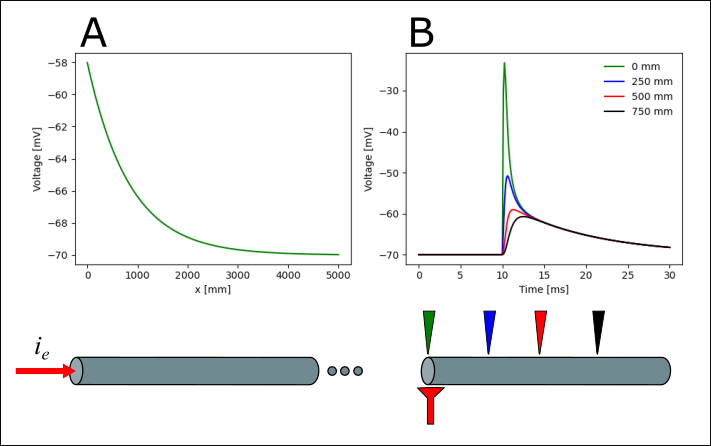
\includegraphics[width=0.7\textwidth]{Figures/Neuron/Cablesims.png}
\caption{\textbf{Stick-neuron responding to transient and constant inputs received in one end.} (A) Finite cable of length $L = 1 \, \text{mm}$ simulated numerically as 100 compartments, and stimulated with an alpha-synapse in the first compartment ($0<x<10 \, \mu\text{m}$). Transient responses shown at different distances from the synapse. The peak response decreases with distance from the synapse, and the time to reach the peak increases with distance from the synapse.
(A) Analytical steady-state solution for semi-infinite cable receiving a constant input $I^{stim} = 0.1 \, \text{nA}$ in a sealed end at $x=0$. The membrane potential decays exponentially with distance from the stimulus site.  (A-B) Parameters choices: $c_m=1\,\mu\text{F}/\text{cm}^2$, $d = 1\, \mathrm{\mu}\text{m}$, $R_a=35.4\, \mathrm{\Omega cm}$, $R_m = 10 \, \mathrm{k\Omega cm^2}$, which gives a length constant $\lambda = 840\, \mathrm{\mu m}$. }
\end{center}
\label{Neuron:fig:Semiinf}
\end{figure}


%%%%%%%%%%%%%%%%%%%%
\subsection{\blue{Cable equation}}
\label{sec:Neuron:cableeq}
\index{Cable equation}
If we in Eq. \ref{Neuron:eq:multipassive} let $L \rightarrow \delta x$, and take the limit $\delta x \rightarrow 0$, we obtain the cable equation (see e.g., \cite**{Sterratt2011}): 

\begin{equation}
c_m \frac{\partial V}{\partial t} = \frac{E_m-V}{R_m} +  \frac{d}{4 R_a}  \frac{\partial^2 V}{\partial x^2}  + \frac{\mathcal{I}^{stim}}{\pi d},
\label{Neuron:eq:cable}
\end{equation}
where we have  introduced the stimulus current per unit length, $\mathcal{I}^{stim}(x,t) = I^{stim}(x,t)/\delta x$ (mA/cm). To improve our analytical understanding of dendritic signaling, it is useful to reformulate the cable equation to:
\begin{equation}
\tau_m \frac{\partial V}{\partial t} = E_m-V +   \lambda^2  \frac{\partial^2 V}{\partial x^2}  + \frac{R_m \mathcal{I}^{stim} }{\pi d},
\label{Neuron:eq:cable2}
\end{equation}
where we have multiplied all terms with $R_m$ and introduced the length constant,
\begin{equation}
\lambda = \sqrt{\frac{d R_m}{4 R_a}} \,\; \text{(cm)}, 
\label{Neuron:eq:lengthconst}
\end{equation}
and the time constant, 
\begin{equation}
\tau_m \equiv R_m c_m  \,\; \text{(ms)}.
\label{Neuron:eq:timeconst}
\end{equation}

The cable equation serves as a continuous version of a passive neural branch (with infinitely many infinitely small compartments), where $\tau_m$ is typical time scale (dimensionless time: $t/\tau$), while $\lambda$  is typical length scale  (dimensionless length: $x/\lambda$) for signals in the cable. If a certain point along the cable is perturbed, so that the potential is shifted from rest to a given value $V$, $\tau_m$ will determine how fast the local potential will dissipate back towards rest, while $\lambda$ will tell us how far the local perturbation will spread along the cable. 

Whereas MC models (Eq. \ref{Neuron:eq:multimain} and \ref{Neuron:eq:multipassive}) generally must be solved numerically, the cable equation allows the spatiotemporal evolution of the membrane potential to be solved analytically for some idealized scenarios. Below, we consider a couple of scenarios that will  make the interpretation of $\tau_m$ and $\lambda$ clearer. 


%%%%%%%%%%%%%%%%%%%%
\subsection{\blue{Steady state solution of the cable equation}}
\label{sec:Neuron:cableSS}
Let find the steady state solution for a semi-infinite cable, receiving a constant current injection at the sealed end in $x=0$ (Fig. \ref{Neuron:fig:Semiinf}B). Since only the end-point receives the stimulus, we may attack this problem by solving eq. \ref{Neuron:eq:cable2} for all other points $x>0$, and then introduce the stimulus current as a boundary condition. 

At steady-state, $\partial V/\partial t = 0$, and Eq. \ref{Neuron:eq:cable2} becomes:
\begin{equation}
0 = E_m-V +  \lambda^2 \frac{\partial^2 V}{\partial x^2}, 
\label{Neuron:eq:semiinf}
\end{equation}
at all points along the cable, except $x=0$. If we introduce the new variable $\Delta{V}=V-E_m$, Eq. \ref{Neuron:eq:semiinf} simplifies to:
\begin{equation}
\frac{d^2 \Delta{V}}{d x^2} -  \frac{1}{\lambda^2} \Delta{V}=0, 
\label{Neuron:eq:semiinf2}
\end{equation}
which has the solution:
\begin{align}
\Delta{V}(x) &= \Delta{V}(0) e^{-x/\lambda} \\
V(x) &= E_m + \big( V(0)-E_m \big) e^{-x/\lambda}.
\label{Neuron:eq:semiinf3}
\end{align}
The general-solution to the equation also has a term containing $e^{+x/\lambda}$, but this was excluded on the count of being unphysical, since it diverges when $x \rightarrow \infty$. 

To get the final solution of the problem, we need to specify the boundary value $V(0)$. This will depend on the stimulus current, and since it only exists in a singular point, we go back to expressing in terms of a total current, $I^{stim}$ (and not as a current per unit length $\mathcal{I}^{stim}$). We introduce it through a boundary condition demanding that the injected current (at $x=0$) must be identical to the axial current in the cable at $x=0$:
\begin{equation}
I^{stim} = - \frac{\pi d^2}{4}\frac{1}{R_a} \frac{\partial V}{\partial x}   \Big|_{x=0}.
\end{equation}
The left hand side is the axial cable current as given by Ohm's law. The multiplication with the cable cross section area (first factor on the left) is used to convert a current density to a total current in the cable. If we insert for $\partial V/\partial x$ (calculated from eq. \ref{Neuron:eq:semiinf3}), and insert eq. \ref{Neuron:eq:lengthconst} for $\lambda$, we can derive the following expression for $V(0)$:
\begin{equation}
V(0) = E_m + R_{\infty}I^{stim}, 
\label{Neuron:eq:firstRinf}
\end{equation}
where we have defined:
\begin{equation}
R_{\infty} = \sqrt{\frac{R_m R_a}{\pi^2 d^3}}.
\label{Neuron:eq:Rinf}
\end{equation}
If we insert eq. \ref{Neuron:eq:firstRinf} into eq. \ref{Neuron:eq:semiinf3}, we obtain our final solution:
\begin{equation}
V(x) = E_m +R_{\infty}I^{stim}  e^{-x/\lambda}.
\label{Neuron:eq:semiinf4}
\end{equation}

The steady state solution to the semi-infinite cable (lotted in Fig. \ref{Neuron:fig:Semiinf}B) is useful as it gives us analytical insight into signals spreading in e.g., passive dendrites. Some insights that can be derived from it is:

\begin{itemize}

\item It follows from eq. \ref{Neuron:eq:firstRinf} that $R_{\infty} = (E_m-V(0))/I^{stim}$, and thus interprets as the steady-state input resistance of the semi-infinite cable. Eq. \ref{Neuron:eq:Rinf} thus shows that the input resistance is proportional to $1/d^{3/2}$, i.e., the input resistance is higher the thinner the dendrite. 

\item Eq. \ref{Neuron:eq:semiinf4} shows that in steady-state, the amplitude will decay exponentially from the injection site and outwards, and will be reduced by a factor $1/e$ over the length $\lambda$. If we put in some typical values in eq. \ref{Neuron:eq:lengthconst}, like a dendritic diameter $d=1$~$\mu$m, a membrane resistance of $R_m=10\;\text{k}\Omega\text{cm}^2$, and an axial resistivity $R_a=35.4\;\Omega\text{cm}$, we get a length constant of $\lambda = 840\; \mu$m. Very long dendrites will thus only to a small degree be affected by the membrane potential in the soma.

\item According to eq. \ref{Neuron:eq:lengthconst}, $\lambda \propto \sqrt{d}$, meaning that signals will spread further the thicker the dendrite.

\item According to eq. \ref{Neuron:eq:lengthconst}, $\lambda \propto \sqrt{R_m/R_a}$ meaning that the signal is facilitated by having a large membrane resistance compared to the axial resistance. 

\end{itemize}

\subsection{\blue{Frequency dependence of the cable length constant}}
\label{sec:Neuron:cablefreq}
As we just saw, the length constant $\lambda$ (eq. \ref{Neuron:eq:lengthconst}) is the length over which the potential falls to a fraction $1/e$ of its boundary value when the finite end of a semi-infinite cable is fixed at a constant potential. As this interpretation depends on a constant, direct-current (DC), boundary condition, $\lambda$ is often referred to as the DC length constant. 

It is possible to derive a corresponding length constant for AC input to a semi-infinite cable \cite**{Pettersen2008a}: 
\begin{equation}
\lambda_{AC} = \lambda \sqrt{ \frac{2}{1+\sqrt{(\omega \tau)^2 + 1}} }.
\label{Neuron:eq:AClambda}
\end{equation}
Here $\tau$ still is the membrane time constant (eq. \ref{Neuron:eq:timeconst}), $\lambda$ is still the DC length constant (eq. \ref{Neuron:eq:lengthconst}), and $\omega = 2\pi f$ is the angular frequency of the the boundary potential.

For a constant boundary condition ($I^{stim} = \text{constant}$ in eq. \ref{Neuron:eq:semiinf4}) or, equivalently, $V(0) = \text{constant}$ in eq. \ref{Neuron:eq:semiinf3}), $\omega$ is zero, and we may verify that $\lambda_{AC}$ becomes identical to the DC length constant $\lambda$. For an AC input, we see that $\lambda_{AC}$ decreases with $\omega$, and for high frequencies $\lambda_{AC} \propto (\omega \tau^{-1/2})$. Thus, low frequency input will tend to travel further in dendritic structures, while high frequency input will affect dendritic structures more locally. 

As we shall see later, an important factor determining the size and shape of extracellular potentials is the distance between inward (sinks) and outward (sources) transmembrane currents. This spatial separation is proportional to the neuronal length constant, and from eq. \ref{Neuron:eq:AClambda} we thus know that the source/sink separation will be larger for low frequency components of the neuronal activity.


\subsection{\blue{GH: Temporal solutions of cable equation}}
\label{sec:Neuron:cabletemp}

In Fig. \ref{Neuron:fig:Semiinf}A we simulated numerically the response of a cylindrical neuron to a  synaptic input in one end. It is possible to show analytically that the passive decay of $V$ following the input-induced peaks can be expressed as a sum of exponentials \cite**{rall1969}:
\begin{equation}
V(x,t) = C_0(x) e^{-t/\tau_0} + C_1(x) e^{-t/\tau_1} + C_2(x) e^{-t/\tau_2} + \ldots, 
\label{Neuron:eq:cabletemporal}
\end{equation}
where the coefficients $C_n(x)$ depend on the distance along the cable, while $\tau_0 = \tau_m = R_m c_m$ is the \emph{membrane time constant} (eq. \ref{Neuron:eq:timeconst}), and the other time constants have successively smaller values ($\tau_0 > \tau_1 > \tau_2 > \ldots$). We will not here present these analytical results in any further detail, but note that the final decay phase, i.e., when $V$ at all locations have coincided, takes place at the slower time scale of the membrane time constant, $\tau_m$ which in the simulation in Fig. \ref{Neuron:fig:Semiinf}A  was 10~ms ($R_m=10\,\text{k}\Omega \text{cm}^2$, and $c_m=1\,\mu\text{F}/\text{cm}^2$). 



%%%%%%%%%%


\section{\blue{Ion concentration dynamics and reversal potentials}}
\label{sec:Neuron:Ions_and_reversals}
\index{Ion concentration dynamics}
MC models as defined in Section \ref{sec:Neuron:Active_multicomp} with membrane mechanisms as specified in Section \ref{sec:Neuron:membranecurrents} give a complete and operational framework for modelling the electrical activity of neurons, which works well for most purposes. The reader may chose to skip the remainder of this chapter, which delves more into the biophysical origin of neural activity. 

Up til this point, we have focused on electrical currents in neurons, but talked little of their biophysical origin, i.e., the ions that carry these electrical currents. For example, action potentials are generated by a transmembrane influx of Na\textsuperscript{+}, which charges up (depolarizes) the neuron, followed by an efflux of K\textsuperscript{+}, which decharges (repolarizes) it. These fluxes are primarily driven by diffusion, and thus depend on the intra- and extracellular solutions having different ionic compositions. 

In the neuron models presented in this chapter, it is implicitly assumed that, despite all these various ionic fluxes, the ion concentrations remain constant. This may seem like a peculiar assumption, but it is often quite good. The reason is that the number of ions crossing the membrane during a brief signal such as an action potential only leads to tiny changes in the ion concentrations on either side of the membrane, so that concentrations changes on a short time scale can be neglected. Since neurons possess a team of homeostatic mechanisms that strive to maintain the trans-membrane ion concentration gradients, the assumption of constant ion concentrations also tends to hold on a longer time scale.  The perhaps most important of these mechanisms is the ATPase pump, which uses energy to pump K$^+$ ions into the neuron and Na$^+$ ions out, thus reversing the ionic exchange that occurs during action potential generation. As a result of this pump, the intracellular space tends to remain comparatively rich in K$^+$, while the extracellular space is tends to remain comparatively rich on Na$^+$. Typical values of ion concentrations of the main charge carriers inside and outside neurons are given in Table \ref{Neuron:tab:ion-concentrations}. 

\begin{table}[h]
%\centering
\caption[]{Major charge carrier concentrations inside/outside a typical mammalian neuron. Concentration values were taken from Table 2-1 in \citeasnoun**{Somjenboka} for neurons in the central nervous system (intracellular) and human cerebrospinal fluid (extracellular). Values vary with species and brain regions. Nernst potentials were computed from Eq. \ref{Neuron:eq:revpots} assuming a body temperature of 309.15 K.
}
\label{Neuron:tab:ion-concentrations}
\begin{tabular}{@{}lcccccc@{}}
\hline
					& 	K$^+$	&	Na$^+$	&	Mg$^{2+}$	  &	Cl$^-$	&	Ca$^{2+}$	 	& HCO3$^-$ 	\\ 
\hline
Intracellular (mM)				    & 125		&		10	&		0.5	&	6.6		&  	6$\times$10$^{-5}$	  & 	18 \\
Extracellular (mM)			           & 2.9			&		147	&		0.7	&	119 		&		1	&	23.3	  	\\
Nernst potential (mV)		    &	-100		&	    	+72	&		+4.5	&	-77		&		+129 	& 	-6.9  	\\
\hline
\end{tabular}
\end{table}

In HH-type models, the ensemble of processes that work to maintain baseline conditions are simply assumed to do their job, and not explicitly modeled. Instead, they are grouped together into the \textit{passive} leakage current $I_L$ (eq. \ref{Neuron:eq:HHleak}), which largely determines the cell's resting potential (see see \cite**{offner1991} for a critical study of this approximation). Below, we shall explain how the ionic concentrations are implicitly present in the HH-formalism as they determine the ionic reversal potentials ($E_x$ in eq. \ref{Neuron:eq:HHform}). We shall also comment on the cases where the assumptions of constant ion concentrations are not applicable. 


\subsection{\blue{Ionic reversal potentials}}
\label{sec:Neuron:Erev}
\index{Reversal potential}
Ion channels are pores in the membrane, some of which are selectively permeable only to specific ions. The ion flux through an open ion channel will be mediated by a combination of (i) diffusion and (ii) electric drift. 

For example, when an K$^+$ channel opens, (i) diffusion will strive to drive K$^+$ out from the neuron, since the intracellular space is more K$^+$-rich than the extracellular space, while electric drift will strive to drive K$^+$ into the neuron, since the membrane potential $V$ (defined as intracellular minus the extracellular potential) tends to be negative ($V \sim - 70$  mV during rest). Initially, the diffusive process will dominate, so that the net flux of K$^+$ is outward. This leads to a gradual decrease (hyperpolarization) of the membrane potential,  and a corresponding gradual increase of the drift component. If the K$^+$ channel stays open, the hyperpolarization will go on until the drift component becomes equal in magnitude to the diffusive component, and the net K$^+$ current becomes zero.

The ionic reversal potential is defined as the membrane potential at which the electrical drift current and diffusive current of a given ion species are in an equilibrium, i.e., they are equal in magnitude but oppositely directed. It can be calculated from the Nernst-Planck equation for electrodiffusion \index{Electrodiffusion}. If we approximate the problem as one-dimensional (in the $z$-direction, perpendicular to the membrane), the Nernst-Planck equation for an ion species $k$ is:

%%%%
\begin{equation}
j_k = j_{k,\text{diff}} + j_{k,\text{drift}} 
=  - P_k \Big(\frac{d[k]}{dz} +  \frac{Fz_k}{RT}  [k] \frac{dV}{dz} \Big), 
\label{Neuron:eq:NP1D}
\end{equation}
%%%%
where the first term is Fick's law for the diffusive flux density along the concentration gradient, and the second term is the electrical drift along the voltage gradient. Here, the membrane's permeability ($P_k$) to ion $k$ has taken the role of the diffusion constant ($D_k$) which appears in the more common form of the Nernst-Planck equation. Furthermore, $z_{k}$ is the valency of ion species $k$, $R = 8.314$ J mol$^{-1}$K$^{-1}$ is the gas constant, $F = 96485.3365$ C/mol is Faraday's constant, and $T$ is the absolute temperature (K). The reversal potential (also called the Nernst-potential) is found by solving for when there is no net flux, i.e., when  $j_{k,\text{diff}} = - j_{k,\text{drift}}$:

\begin{equation}
\frac{1}{[k]} \frac{d[k]}{dz} = - \frac{Fz_k}{RT}  \frac{dV}{dz}.
\end{equation}
We may multiply both sides by $dz$ and re-arrange this to get:
\begin{equation}
-dV = \frac{RT}{Fz_k}  \frac{d[k]}{[k]}.
\end{equation}
If we integrate this from the inside to the outside of the membrane, we get:
\begin{align}
-\int_{V_{\text{in}}}^{V_{\text{out}}}  dV &= \frac{RT}{Fz_k}  \int_{[k]_{\text{in}}}^{[k]_{\text{out}}} \frac{d[k]}{[k]} \rightarrow \\
V_{\text{in}}-V_{\text{out}} &= \frac{RT}{Fz_k} ln \frac{[k]_{\text{out}}} {[k]_{\text{in}}} \rightarrow \\
E_k & =  \frac{RT}{Fz_k}  ln \frac{[k]_{\text{out}}} {[k]_{\text{in}}} 
\label{Neuron:eq:revpots}
\end{align}
where the last equality follows from the definition of $E_k$ as the membrane potential $V_{\text{in}}-V_{\text{out}}$ for which the the net flux (in Eq. \ref{Neuron:eq:NP1D}) is zero. Eq. \ref{Neuron:eq:revpots} was used to compute the reversal potentials listed in Table \ref{Neuron:tab:ion-concentrations}. 

As ion concentrations are generally assumed to remain constant in HH-type models, the reversal potentials are also assumed to be constant. As a consequence, one typically do not think that much about ionic concentrations when constructing such models, but simply use values for $E_k$ based or empirical measurements of the potential at which a certain membrane current reverses, i.e., becomes zero.


\subsection{\blue{The Goldman-Hodgkin-Katz equation}}
\label{sec:Neuron:GHK}
\index{Goldman-Hodgkin-Katz equation}
Eq. \ref{Neuron:eq:NP1D} defined the reversal potential for an individual ion species, which is relevant for modeling ion-specific ion channels. To calculate the reversal potential for a non-specific ion channel, we need to express all the individual ion currents separately, and compute the value of $V$ for which they sum to zero. 

If we combine Eq. \ref{Neuron:eq:NP1D} with the assumptions that (i) ions cross the membrane independently, and (ii) that the electrical field within the membrane is constant, we can derive the Goldman-Hodkgkin-Katz (GHK) equation for the membrane currents (see e.g., \cite**{hodgkin1949,johnston1994foundations}):
\begin{equation}
I_\text{k} = P_k z_k F \frac{z_k F V}{R T} \Big( \frac{[k]_\text{in}-[k]_\text{out} e^{-z_k F V/RT}} {1-e^{-z_k F V/RT}} \Big).
\label{Neuron:eq:GHK}
\end{equation}

An example of a non-specific ion channel is the passive leakage current which has a permeability to all ion species simultaneously, so that its reversal potential ($E_L$ in Eq. \ref{Neuron:eq:HHleak}) will depend on all ion concentrations. If we assume that only the three most abundant charge carriers (K$^{+}$, Na$^{+}$ and Cl$^{-}$) contribute, and that they have leak permeabilities $P_K$, $P_{Na}$ and $P_{Cl}$, we can derive from eq. \ref{Neuron:eq:GHK} that they are in equilibrium at the potential:
\begin{equation}
E_L = \frac{R T}{F} 
\ln \frac{P_\text{K} [K]_\text{out}+P_\text{Na} [Na]_\text{out} + P_\text{Cl} [Cl]_\text{in}}
           {P_\text{K} [K]_\text{in}+P_\text{Na} [Na]_\text{in} + P_\text{Cl} [Cl]_\text{out}}.
\label{Neuron:eq:Eleak_GHK}
\end{equation}

Looking at eq. \ref{Neuron:eq:GHK}, we see that the transmembrane currents are nonlinear functions of both the ionic concentrations $[k]$ in the intra and extracellular space, and the membrane potential $V$. In comparison, the transmembrane currents used in the HH-type formalism (eq. \ref{Neuron:eq:HHform}), which are proportional to the driving force $(V-E_k)$, are linearized (sometimes called quasi-Ohmic) versions of the Goldman-Hodkgkin-Katz equation. The HH-form (eq. \ref{Neuron:eq:HHform}) is generally deemed as sufficient for modeling most ion channels, because it gives good predictions of the membrane currents. Ion concentrations and ionic reversal potentials are then assumed to be constant.


\subsection{\blue{Intracellular Calcium dynamics}}
\label{sec:Neuron:Calcium}
\index{Calcium dynamics}
While most ion concentrations are assumed to be constant in HH-based models, it is common to make an exception for Ca$^{2+}$. The main reason for this is that the intracellular Ca$^{2+}$ concentration ($\mathrm{[Ca]_i}$) is very low compared to that of the other ion species (Table \ref{Neuron:tab:ion-concentrations}). Unlike for the other ion species,  $\mathrm{[Ca]_i}$, can therefore change quite dramatically on a short time scale, e.g., during the opening of Ca$^{2+}$ channel. 

The motivations for modeling $\mathrm{[Ca]_i}$ are several. Firstly, to accurately model currents through Ca$^{2+}$ channels, the concentration dependent GHK formalism (eq. \ref{Neuron:eq:GHK}) is often used (see e.g., \cite**{Destexhe1994,Zhu1999,Halnes2011}), and one then needs an expression for $\mathrm{[Ca]_i}$. Secondly, modeling $\mathrm{[Ca]_i}$ could be motivated by the aim to reproduce data from Ca$^{2+}$ imaging experiments. Thirdly, Ca$^{2+}$ does not only act as a charge carrier in neurons, but is also a second messenger, which means that it can trigger a number of intracellular chemical processes, including the gating of Ca$^{2+}$ activated ion channels. 

When Ca$^{2+}$ dynamics is included in HH-based models, it is usually to account for the activation of ion channels that instead of being voltage gated, open or close as a function of $\mathrm{[Ca]_i}$. The kinetics scheme for voltage gated ion channels (\ref{Neuron:eq:HHgate}) \index{Calcium gated ion channels} is then replaced with one dependent on $\mathrm{[Ca]_i}$:

\begin{equation}
\frac{dx(V,t)}{dt} = \frac{x_{\infty}(\mathrm{[Ca]_i}) - x}{\tau_x(\mathrm{[Ca]_i}},  \, \text{for } x = \{m,h\},
\label{Neuron:eq:Cagate}
\end{equation}
and the $\mathrm{[Ca]_i}$ in a neuronal compartment is typically modeled using a simplified framework on the form:
\begin{equation}
\frac{d\mathrm{[Ca]_i}}{dt} = \gamma i_{Ca} - \frac{\mathrm{[Ca]_i}-\mathrm{[Ca]_{i,0}}}{\tau_{Ca}}, 
\label{Neuron:eq:Cadynamics}
\end{equation}
where a transmembrane Ca$^{2+}$ current ($i_{Ca}$ is converted to a change in $\mathrm{[Ca]_i}$ by the conversion factor $\gamma$, which is proportional to the surface to volume ratio of the neuronal compartment where $\mathrm{[Ca]_i}$ is defined. In addition, the last term in eq. \ref{Neuron:eq:Cadynamics} represents the summed activity of a number of extrusion mechanisms that will make $\mathrm{[Ca]_i}$ decay towards some baseline value $\mathrm{[Ca]_{i,0}}$ with a time constant $\tau_{Ca}$ (see e.g. \cite**{Sterratt2011}).

To use a simple model as in eq. \ref{Neuron:eq:Cadynamics} might not be meaningful when it comes to model the more abundant ion species (K$^{+}$, Na$^{+}$ and Cl$^{-}$). One reason is that eq. \ref{Neuron:eq:Cadynamics} only considers the intracellular concentration. This makes sense for Ca$^2+$, since the intracellular concentration is much smaller than the extracellular concentration, so that $\mathrm{[Ca]_i}$ can experience dramatical relative changes while the extracellular concentration remains approximately constant. The same does not hold for the more abundant species, for which the concentrations are of the same order of magnitude on both sides of the membrane. Another reason is that eq. \ref{Neuron:eq:Cadynamics} is local in the sense that the concentration is affected exclusively by transmembrane ionic currents. In reality, also the axial intracellular currents are carried by ions, especially by the more abundant ones \cite**{Qian1989}. A complete and consistent model of ion concentration dynamics would thus need to account for electrodiffusive ion concentration dynamics both in the intra- and extracellular space. Such models exist (see e.g., \cite**{Saetra2020,ellingsrud2020}), but they are generally computationally heavy, and not based on the MC framework that we have presented here. 


\section{\blue{Underlying assumptions in multicompartment models}}
\label{sec:Neuron:HHCassumptions}
As the final part of this chapter, we summarize the key assumptions that the standard MC framework is based upon.

\begin{itemize}
\item HH-type ion channels are simplified approximations of the electrophysiological dynamics of ion channel gating. There exist more detailed ion channel models based on a formalism more compatible with statistical physics and thermodynamics \cite**{Destexhe2010}, or even more detailed, Markov-type formalism based on single-channel recordings \cite**{sakmann2013}.

\item Being based on the cable equation, MC models assume that the neuronal morphology is well represented by a one-dimensional, branching cable, meaning that radial components of intracellular currents are neglected. See e.g.,\citeasnoun**{lindsay2004maxwell} for a critical study of this approximation.

\item Eq. \ref{Neuron:eq:multimain} was derived under the assumption that the extracellular potential ($V_e$) is zero. Generally, $V_e$ is much smaller than the membrane potential $V$, but some (so-called \textit{ephaptic}) effects \index{Ephaptic effects} of $V_e$ on neurodynamics could occur \cite**{Holt1999,anastassiou2015,Tveito2017}. Such effects are not accounted for in the standard MC models.

\item As we explained in Section \ref{sec:Neuron:Ions_and_reversals}, the concentrations of the main charge carriers are constant are assumed to be constant in standard MC models. As the main ion concentrations change little during normal neuronal activity, this assumption is often warranted. However, there exist scenarios when this is not true, and dramatic changes in ion concentrations is a trademark of several pathological conditions, such as epilepsy, stroke and spreading depression \cite**{Somjen2001,Zandt2015,Ayata2015}. When concentrations change, so will ionic reversal potentials and thus the dynamical properties of neurons. Standard MC models are not suited to model neurons under such conditions.

\end{itemize}

